\chapter{Ciudades y versiones del grafo}\label{cap:versiones}

Los algoritmos del viajante no trabajan sobre el grafo vial de 180.000 nodos, sino sobre un grafo mucho más pequeño cuyos nodos son las \emph{ciudades} y cuyas aristas son las
distancias entre ellas. Este capítulo explica qué ciudades se eligen, cómo se calculan esas distancias y cómo se obtienen, a partir de una única red, las 480 versiones del problema que
se estudian.

\section{Las ciudades}

El conjunto de ciudades son \textbf{75 municipios de la España peninsular}: las 47 capitales de provincia peninsulares (50 provincias menos las capitales insulares, Palma, Las Palmas de Gran Canaria y Santa Cruz de Tenerife)
y los 28 municipios peninsulares de más de 100.000 habitantes que no son capitales (de los 62 que hay en la península, 34 ya lo son). Se excluyen los municipios insulares de más de 100.000 habitantes (La Laguna y Telde)
porque la red vial peninsular no los conecta. De este modo se dispone de dos conjuntos anidados, \texttt{capitales} (47 ciudades) y \texttt{capitales\_y\_100k} (75 ciudades), que permiten estudiar cómo crece el problema.

\begin{figure}[htbp]
  \centering
  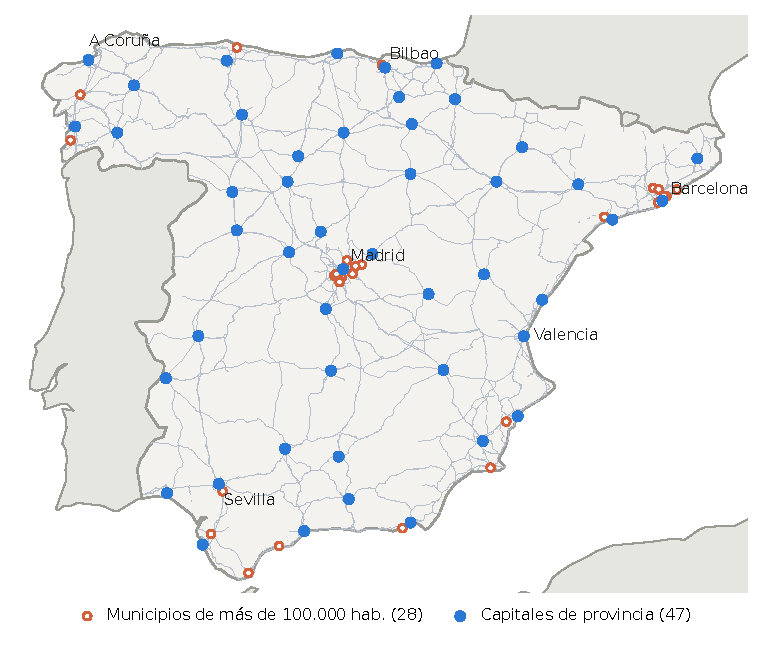
\includegraphics[width=0.78\linewidth]{red_ciudades.pdf}
  \caption{Las 75 ciudades del estudio sobre la red de autovías y vías rápidas (fondo gris). Los círculos azules son las 47 capitales de provincia; los círculos naranjas, los 28 municipios de más de 100.000 habitantes que no son capitales.}
  \label{fig:ciudades}
\end{figure}

\paragraph{Fuentes.} La lista de capitales y la población proceden del INE (\emph{Cifras oficiales de población de los municipios españoles: Revisión del Padrón Municipal}, datos a 1 de enero de 2025,
publicados el 11 de diciembre de 2025 en el BOE-A-2025-25362). La comunidad autónoma de cada ciudad se asignó con las tablas por provincia del INE. Las \textbf{coordenadas} proceden de los nodos
\texttt{place=city} o \texttt{place=town} de OpenStreetMap, el centro de cada núcleo urbano; no son una fuente oficial. Una primera geocodificación con Nominatim devolvía la provincia en lugar del
municipio para algunas capitales (Guadalajara, Palencia\dots) y el centro del término municipal en otras (Almería quedaba 14~km desplazada), por lo que se sustituyó por los nodos del propio extracto.

\section{De las ciudades a la red}

Cada ciudad se asocia al \emph{nodo de carretera más cercano}, mediante una búsqueda en un árbol $k$-d (\texttt{cKDTree} de SciPy) sobre coordenadas convertidas a kilómetros. Si ese nodo está a más de
$X=10$~km, la ciudad no está realmente conectada a esa versión de la red y se deja fuera de ella, registrando su distancia. Esto solo ocurre en una versión (sección~\ref{sec:redes}). La distancia entre la ciudad y su nodo
\emph{no} se suma a las distancias: es una simplificación del acceso que afecta por igual a todos los algoritmos.

\section{Tablas de distancias}

Para dos ciudades $a$ y $b$ con nodos asociados $u_a$ y $u_b$, la distancia entre ellas es la del camino mínimo en el grafo vial:
\begin{equation}\label{eq:dijkstra}
  D(a,b)\;=\;\min_{P:\,u_a\to u_b}\ \sum_{e\in P} w(e),
\end{equation}
donde $P$ recorre las aristas respetando los sentidos y $w$ es la longitud (\texttt{length}, que se convierte a kilómetros) o el tiempo de viaje (\texttt{travel\_time}). Se calcula con el algoritmo de Dijkstra~\cite{dijkstra1959} (implementación de SciPy) desde cada una de las 75 ciudades.
Como los sentidos únicos hacen que $D(a,b)\neq D(b,a)$, la tabla es asimétrica: por ejemplo, de Madrid a Sevilla hay 502~km y de Sevilla a Madrid, 517~km. Para el caso sin sentidos únicos se ignoran las direcciones y cada tramo cuesta lo
que la más barata de sus dos direcciones.

Los caminos mínimos cumplen la desigualdad triangular~\eqref{eq:triangular} por construcción, de modo que todas las versiones del problema son métricas (las no dirigidas, además, simétricas). Esto es lo que permite aplicar
Christofides con garantía a las versiones no dirigidas.

\section{Las versiones del problema}\label{sec:versiones}

Una \emph{versión} se define con cinco elecciones (tabla~\ref{tab:parametros}). Cada versión se carga con una función \texttt{cargar\_version(\dots)} que devuelve un grafo de NetworkX cuyos nodos son las ciudades y
cuyo peso \texttt{peso} es la distancia.

\begin{table}[htbp]
  \centering
  \caption{Parámetros que definen una versión del problema.}\label{tab:parametros}
  \small
  \begin{tabularx}{\linewidth}{@{}l X@{}}
    \toprule
    Parámetro & Valores \\
    \midrule
    \texttt{aristas} & \texttt{completo} (8 tipos de vía), \texttt{autovias\_principales} (sin secundarias), \texttt{solo\_autovias} y \texttt{sin\_autovias}. \\
    \texttt{nodos} & \texttt{capitales} (47 ciudades) o \texttt{capitales\_y\_100k} (75 ciudades). \\
    \texttt{ambito} & \texttt{espana} o una de las 15 comunidades autónomas peninsulares. \\
    \texttt{peso} & \texttt{km} (kilómetros) o \texttt{tiempo} (segundos, el registrado en el grafo). \\
    \texttt{general} & \texttt{multigrafo\_dirigido}, \texttt{grafo\_dirigido}, \texttt{multigrafo\_no\_dirigido} o \texttt{grafo\_simple\_no\_dirigido}. \\
    \bottomrule
  \end{tabularx}
\end{table}

\subsection{Cuántas versiones hay}

Combinando 4 redes, 2 pesos y dirigido o no dirigido se obtienen \textbf{16 tablas} de $75\times 75$ (en total, 0,9~MB). Cada versión es un \emph{trozo} de una de esas tablas, las filas y columnas
de las ciudades que correspondan. Guardar 480 grafos de carreteras ocuparía decenas de gigabytes; así, en cambio, quienes programan los algoritmos no necesitan el grafo grande.

El catálogo contiene \textbf{480 versiones}, que corresponden a \textbf{240 grafos de ciudades distintos}, porque entre dos nodos el camino mínimo solo usa la arista más barata, de modo que el multigrafo y el grafo simple
dan exactamente la misma tabla. De los 240 grafos, 32 son de toda España (44 a 75 ciudades) y 208 son regionales (4 a 13 ciudades). Las versiones regionales usan \emph{toda la red} (el mejor camino entre dos ciudades de una
comunidad puede salir de ella) y requieren un mínimo de $N_{\min}=4$ ciudades, lo que da 5 conjuntos de capitales (Andalucía, Castilla y León, Castilla-La Mancha, Cataluña y Galicia) y 8 de capitales más municipios de más de 100.000 habitantes
(los anteriores más Madrid, Comunidad Valenciana y País Vasco). Los tamaños regionales son 4, 5, 6, 8, 9, 11 y 13 ciudades, y son los que permiten aplicar los algoritmos exactos de enumeración a datos reales.

\subsection{Las cuatro versiones de carreteras}\label{sec:redes}

Las cuatro redes se obtienen filtrando aristas del grafo base y conservando, en cada caso, la mayor componente fuertemente conexa (tabla~\ref{tab:redes}).

\begin{table}[htbp]
  \centering
  \caption{Lo que queda en cada versión de carreteras.}\label{tab:redes}
  \small
  \begin{tabularx}{\linewidth}{@{}l r r r r X@{}}
    \toprule
    Red & Nodos & Aristas & Km & \makecell[r]{Nodos\\descartados} & Ciudades fuera \\
    \midrule
    \texttt{completo} & 179.594 & 309.250 & 182.760 & 0 & ninguna \\
    \texttt{autovias\_principales} & 115.476 & 190.221 & 111.121 & 5.885 & ninguna \\
    \texttt{solo\_autovias} & 19.239 & 24.450 & 28.921 & 14.027 & 3: Salamanca (62,7~km), Badajoz (50,5~km), Cuenca (39,6~km) \\
    \texttt{sin\_autovias} & 146.903 & 256.301 & 140.040 & 8.464 & ninguna \\
    \bottomrule
  \end{tabularx}
\end{table}

\texttt{autovias\_principales} elimina las carreteras secundarias; \texttt{solo\_autovias} deja únicamente autopistas y autovías; \texttt{sin\_autovias} excluye autopistas y autovías (la red «para ir por carreteras convencionales»).
En \texttt{solo\_autovias}, tres ciudades quedan a más de 10~km de la red y se dejan fuera, de modo que esa versión tiene 44 o 72 ciudades en lugar de 47 o 75.

\section{Decisiones de diseño}

\begin{itemize}
  \item \textbf{Bicicleta y a pie no son versiones aparte.} Con velocidad constante, el tiempo es proporcional a la distancia, así que el camino más corto y el recorrido óptimo coinciden con los de kilómetros.
        El caso «a pie o en bici» es \texttt{sin\_autovias} en kilómetros; para horas basta dividir (entre 20 en bicicleta, entre 5 a pie). Descartamos esas versiones para no duplicar resultados idénticos.
  \item \textbf{Las ciudades fuera de la red no se «arreglan».} Como ocurre con las islas, el viajante no puede visitar una ciudad desconectada; se registra y se deja fuera. Por eso Castilla y León pasa de 9 a 8 capitales en \texttt{solo\_autovias}.
  \item \textbf{Modelo no dirigido.} Al ignorar los sentidos únicos, cada tramo vale lo que la más barata de sus dos direcciones. Un atajo por una rampa en contradirección es un efecto pequeño, pero existe.
  \item \textbf{Una sola red maestra.} Todo se deriva del grafo base; así cualquier cambio en los criterios (por ejemplo, el umbral de 10~km) se propaga recalculando las 16 tablas, unos dos minutos.
\end{itemize}

\section{Comprobaciones}

Sobre las 16 tablas se comprueba que las distancias son finitas y no negativas, que la diagonal es cero, que las tablas no dirigidas son simétricas, que la distancia no dirigida nunca supera a la dirigida y que se cumple la
desigualdad triangular (con una tolerancia de 0,01 por el redondeo a tres decimales al guardar). Además, se cargaron sin error las 480 versiones del catálogo.
